%% ============================================================
%% Applying OAuth 2.1 Token Exchange with Nested Actor Claims
%% to MCP Workflows — Full Version (15+ pages)
%%
%% Compile: pdflatex paper_nac_mcp_full.tex  (run twice)
%% Requires: IEEEtran.cls, tikz, pgfplots, booktabs, multirow
%% ============================================================
\documentclass[journal]{IEEEtran}
\IEEEoverridecommandlockouts

%% — packages —
\usepackage{cite}
\usepackage{amsmath,amssymb,amsfonts}
\usepackage{graphicx}
\usepackage{textcomp}
\usepackage{xcolor}
\usepackage{booktabs}
\usepackage{url}
\usepackage{hyperref}
\usepackage{listings}
\usepackage{multirow}
\usepackage{array}
\usepackage{tikz}
\usepackage{pgfplots}
\usepackage{pgfplotstable}
\usepackage{colortbl}
\usepackage{tabularx}
\usepackage{footnote}
\usepackage{balance}

\usetikzlibrary{arrows.meta, shapes, positioning, fit, backgrounds, patterns,
                decorations.pathreplacing, calc}
\pgfplotsset{compat=1.18}

\hypersetup{colorlinks=true,linkcolor=blue,citecolor=blue,urlcolor=blue}

\definecolor{basecolor}{HTML}{E07B54}   % warm orange — baseline/insecure
\definecolor{seccolor}{HTML}{4C9BE8}    % cool blue   — NAC/secure
\definecolor{parcolor}{HTML}{5DBB7A}    % green       — parallel / blocked
\definecolor{warncolor}{HTML}{E74C3C}   % red
\definecolor{lightgray}{HTML}{F5F5F5}
\definecolor{midgray}{HTML}{CCCCCC}
\definecolor{darkblue}{HTML}{2C3E50}

\lstset{
  basicstyle=\scriptsize\ttfamily,
  breaklines=true,
  frame=single,
  captionpos=b,
  xleftmargin=1em,
  xrightmargin=0em,
  numbers=left,
  numberstyle=\tiny\color{gray},
  numbersep=5pt,
  keywordstyle=\color{blue}\bfseries,
  commentstyle=\color{green!60!black},
  stringstyle=\color{red!80!black},
}

%% ============================================================
\begin{document}

\title{Applying OAuth 2.1 Token Exchange with Nested Actor Claims\\
to MCP Workflows: Design, Implementation, and\\
Empirical Security Evaluation}

\author{\IEEEauthorblockN{[Author Name]}
\IEEEauthorblockA{\textit{[Department]} \\
\textit{[Institution]}\\
[City, Country]\\
[email@institution.edu]}
\and
\IEEEauthorblockN{[Co-Author Name (if any)]}
\IEEEauthorblockA{\textit{[Department]}\\
\textit{[Institution]}\\
[City, Country]\\
[email@institution.edu]}}

\maketitle

%% ============================================================
\begin{abstract}
The Model Context Protocol (MCP), introduced by Anthropic in November 2024 and adopted by OpenAI, Google DeepMind, and the Linux Foundation's Agentic AI Foundation by 2025, defines the emerging standard for connecting large language model (LLM) agents to external tools and services. As MCP deployments scale to multi-agent, multi-service orchestration, a pervasive security anti-pattern has emerged: \textit{token passthrough}, in which the orchestrating AI assistant forwards the user's original OAuth access token unchanged to every downstream service it invokes. Token passthrough simultaneously violates three independent security properties: \textbf{audience binding} (a token valid for one service is accepted at others), \textbf{scope attenuation} (all permissions are forwarded regardless of what each service requires), and \textbf{delegation chain visibility} (the audit trail cannot attribute which agent made which call). The MCP security specification explicitly identifies the resulting vulnerability as the \textit{Confused Deputy Problem}. We propose applying RFC 8693 (OAuth 2.0 Token Exchange) with Nested Actor Claims (NAC) as a principled, standard-compliant remedy. At each delegation hop, the AI orchestrator exchanges the parent token for a fresh, narrowly scoped child token; each child token carries a service-specific \texttt{aud} claim, an attenuated \texttt{scope}, a nested \texttt{act} claim recording the full delegation chain, and a one-time-use \texttt{jti} revoked in Redis after first use. We present the first empirical implementation and evaluation of RFC 8693 NAC specifically for MCP multi-agent workflows. Our reference implementation, built on Python 3.10, FastAPI, the MCP SDK, and Claude Sonnet as the real LLM planner, blocks all four concrete attack vectors—scope escalation, lateral movement, token replay, and identity confusion—with 100\% block rate across 30 experimental trials each. An ablation study (six enforcement configurations × four attack vectors × 30 trials = 720 data points) confirms that each security property is independently necessary: no single property suffices to block all attacks. Measured latency overhead is $+37.7\%$ ($+43$ ms mean) on a single-machine demo setup, with an estimated production overhead of $7$--$15\%$ using co-located Redis and multi-worker OAuth services. Token size overhead from the \texttt{act} claim is at most $+8.2\%$ per hop. Per-hop exchange cost scales linearly at $\approx 2.15$ ms per additional delegation hop, validating the theoretical claim of $O(k)$ overhead for $k$-hop chains. These results demonstrate that RFC 8693 NAC provides provable, measurable, and deployable security for MCP multi-agent systems at acceptable production cost.
\end{abstract}

\begin{IEEEkeywords}
Model Context Protocol, OAuth 2.0, Token Exchange, Nested Actor Claims, Confused Deputy, Multi-Agent AI, Access Control, Delegation Chains, LLM Security, OWASP GenAI
\end{IEEEkeywords}


%% ============================================================
\section{Introduction}
\label{sec:introduction}
%% ============================================================

Autonomous AI systems are undergoing a fundamental architectural shift: from single-model, single-context chatbots toward distributed multi-agent orchestrators that decompose complex user tasks and invoke specialized downstream services. A software engineer asks an AI assistant to ``review my calendar, draft a meeting summary, send it to the team, and post a Slack update.'' Behind this single user request lies a coordinated sequence of API calls to four separate services—calendar, document store, email, and messaging—each requiring authorization.

The \textit{Model Context Protocol} (MCP) \cite{mcp_spec}, introduced by Anthropic in November 2024, has rapidly become the de facto open standard for this architecture, adopted by OpenAI (March 2025), Google DeepMind, and subsequently donated to the Linux Foundation's Agentic AI Foundation (December 2025) \cite{mcp_wiki}. MCP defines how an AI \textit{host} exposes tools to an agent and how \textit{server} services expose tools to the host via a standardized JSON-RPC 2.0 transport. By early 2025, analysis of publicly available MCP servers revealed that 43\% contained command injection vulnerabilities and that real-world exploitation had already occurred, with a single critical vulnerability (CVE-2025-6514, CVSS 9.6) affecting over 558,000 installations \cite{mcp_sec_medium_2025}.

Within this environment, one implementation decision quietly undermines the security of every service the AI agent touches: \textbf{token passthrough}—the practice of forwarding the user's original OAuth access token unchanged to every downstream service. This is not a hypothetical risk. It is the natural default for developers integrating MCP without explicit security guidance, and security researchers \cite{cosai_mcp}, industry analysts \cite{checkmarx_mcp}, and the MCP specification itself \cite{mcp_security} have all called it out as the primary OAuth vulnerability in agentic deployments.

Token passthrough enables the \textit{Confused Deputy Problem} \cite{hardy1988}—a 35-year-old vulnerability concept now manifesting in a new context. The deputy (the AI assistant) holds broad authorization that was intended only for its own use, but downstream services cannot distinguish between the assistant legitimately exercising its own permissions and an attacker exploiting those permissions. The Coalition for Secure AI (CoSAI) \cite{cosai_mcp} recommends explicitly: ``don't pass through OAuth tokens directly. Use token exchange (RFC 8693) to maintain full accountability and prevent confused deputy attacks.''

This paper makes the following contributions:

\begin{enumerate}
  \item We formally characterize the token passthrough anti-pattern in MCP and identify three independent security properties it violates (Section~\ref{sec:problem}).
  \item We propose RFC 8693 Token Exchange with Nested Actor Claims as the solution, describe the per-hop exchange architecture, and prove it eliminates all three violations simultaneously (Section~\ref{sec:solution}).
  \item We present the first complete, empirical implementation of RFC 8693 NAC for MCP multi-agent workflows, including a working OAuth 2.1 authorization server, MCP-compliant hub and worker services, a real LLM planner (Claude Sonnet), and a Redis-backed JTI revocation store (Section~\ref{sec:implementation}).
  \item We evaluate the implementation against four concrete attack vectors with an ablation study producing 720 data points, demonstrating that each security property is independently necessary (Section~\ref{sec:evaluation}).
  \item We quantify per-hop cost linearity, measure production overhead, and provide a decomposed overhead analysis showing Redis contributes only $\approx 2\%$ of total overhead (Section~\ref{sec:evaluation}).
\end{enumerate}

%%
%% IMAGE PROMPT 1
%% Title: "The Problem vs. The Solution — Token Passthrough vs. NAC"
%% Prompt for AI image generator:
%% "Technical architecture diagram split into two halves. LEFT HALF labeled 'Token Passthrough (Insecure)': 
%%  a human user icon at top connected by arrow to a central AI robot server hub, which sends the SAME 
%%  orange token to Calendar, Documents, Email, and Slack services arranged in a grid, with a red 
%%  warning shield. RIGHT HALF labeled 'NAC-Secured (RFC 8693)': same human icon connected to the 
%%  same AI hub, but now the hub has a golden exchange icon and sends DIFFERENT colored tokens 
%%  (blue, green, purple, teal) each labeled with their specific service name, with a green 
%%  checkmark shield. Clean flat design, white background, professional technical style."
%%
%% (Replace \includegraphics below with your generated image)


%% ============================================================
\section{Background and Definitions}
\label{sec:background}
%% ============================================================

\subsection{Large Language Models and Agentic AI}

A \textit{Large Language Model} (LLM) is a neural network trained on vast text corpora to predict and generate human-like text \cite{vaswani2017}. Modern LLMs such as GPT-4 \cite{openai2023gpt4}, Claude \cite{anthropic_claude}, and Gemini exhibit emergent capabilities including complex reasoning, tool use, and multi-step planning. \textit{Agentic AI} refers to systems in which an LLM autonomously selects and executes actions—including calling external APIs, reading and writing files, and managing state—to achieve a user-specified goal \cite{wang2024survey}.

The \textit{ReAct} paradigm \cite{yao2022react} interleaves reasoning traces with action calls, enabling an LLM to iteratively plan, execute, observe, and re-plan. This is the computational model underlying MCP tool use: the LLM reasons about which tool to call, calls it, observes the result, and continues. Our reference implementation uses Claude Sonnet via the Anthropic Messages API in a ReAct loop over live MCP tools when \texttt{ANTHROPIC\_API\_KEY} is set.

\subsection{OAuth 2.1 and Bearer Tokens}

\textit{OAuth 2.0} \cite{rfc6749}, formalized in RFC 6749 (2012), is the industry-standard delegated authorization framework. A resource owner (user) authorizes a client (application) to access protected resources on their behalf, without sharing credentials. OAuth 2.1 \cite{oauth21} consolidates security best practices from OAuth 2.0, mandating PKCE for all clients and deprecating the implicit grant.

An \textit{access token} is a bearer credential—any party in possession of the token can use it. RFC 9068 \cite{rfc9068} profiles access tokens as JSON Web Tokens (JWTs) \cite{rfc7519} containing standardized claims: \texttt{iss} (issuer), \texttt{sub} (subject/user), \texttt{aud} (audience/intended recipient), \texttt{scope} (permissions), \texttt{exp} (expiry), and \texttt{jti} (unique token ID). The \texttt{aud} claim is a security boundary: a token issued for Service A should be rejected by Service B.

\subsection{JSON Web Tokens (JWT)}

\textit{JSON Web Tokens} (RFC 7519) \cite{rfc7519} encode claims as a base64url-encoded JSON object, digitally signed (JWS) or encrypted (JWE). RSA-2048/RS256 signatures provide asymmetric security: the issuer signs with a private key; any party can verify with the corresponding public key, but only the issuer can create valid tokens. Our implementation uses RSA-2048 with RS256; workers hold only the public key (\texttt{NAC\_PUBLIC\_ONLY=1}) and physically cannot forge tokens.

\subsection{RFC 8693: OAuth 2.0 Token Exchange}

RFC 8693 \cite{rfc8693} (published January 2020) defines a protocol by which an authorized client exchanges one token for another with different properties. The token exchange request is an HTTP POST to the token endpoint with:

\begin{lstlisting}[language={},caption={RFC 8693 token exchange request parameters}]
grant_type=urn:ietf:params:oauth:
  grant-type:token-exchange    (mandatory)
subject_token=<T_parent>       (token being exchanged)
subject_token_type=...access_token
audience=<target_service>      (intended audience)
scope=<requested_scopes>       (may be narrower)
actor_token=<actor_identity>   (the exchanger)
actor_token_type=...jwt
requested_token_type=...access_token
\end{lstlisting}

The authorization server validates the subject token, enforces that requested scopes do not exceed the subject token's scopes (\textit{scope attenuation}), and issues a fresh token with a narrowed \texttt{aud} and \texttt{scope}. The \texttt{act} claim in the new token records the identity of the actor performing the exchange. Nested \texttt{act} claims form a \textit{delegation chain}: the outermost \texttt{act} represents the current actor; inner \texttt{act} claims represent prior actors in reverse chronological order \cite{rfc8693}.

As illustrated in Figure~\ref{fig:actchain}, a three-hop chain (Alice $\to$ Hub $\to$ Calendar $\to$ External-API) produces:

\begin{lstlisting}[language={},caption={Nested act claim for 3-hop delegation},
                   label={lst:actchain}]
{
  "sub": "alice",
  "aud": "external-api-service",
  "scope": "calendar:read",
  "act": {
    "sub": "calendar-service",
    "act": {
      "sub": "assistant-hub"
    }
  }
}
\end{lstlisting}

\subsection{The Model Context Protocol}

MCP \cite{mcp_spec} defines a client-server protocol for AI tool use, transported over JSON-RPC 2.0 with Server-Sent Events (SSE) or Streamable HTTP. An \textit{MCP server} exposes:
\begin{itemize}
  \item \textbf{Tools}: callable functions with JSON Schema input definitions
  \item \textbf{Resources}: data sources the server can provide
  \item \textbf{Prompts}: template instructions
\end{itemize}

An \textit{MCP client} (the agent) connects via SSE, calls \texttt{initialize}, lists tools, and invokes them. The MCP authorization specification requires bearer tokens in the \texttt{Authorization: Bearer} HTTP header. MCP defines two primary roles:
\begin{itemize}
  \item \textbf{Host}: the AI application (e.g., Claude Desktop, a custom application)
  \item \textbf{Server}: the MCP-compliant service (e.g., a calendar integration)
\end{itemize}

In a multi-service scenario, the assistant hub functions as both a server (to the agent) and a client (to worker services). This intermediary role is the exact topology that creates the Confused Deputy attack surface.

\subsection{Redis for Distributed JTI Revocation}

\textit{Redis} \cite{redis} is an open-source, in-memory data structure server providing sub-millisecond key-value operations. It is the industry-standard backend for distributed token revocation, session management, and rate limiting. The RFC 8693 token lifecycle (issue $\to$ register jti $\to$ use $\to$ revoke jti) maps naturally to Redis \texttt{SET}/\texttt{GET} operations with TTL-based automatic expiry. Each JTI operation completes in $\approx 0.1$ ms on co-located hardware, compared to $\approx 65$ ms for file-based locking on Windows, which is why Redis is essential for keeping NAC overhead within acceptable bounds.

\subsection{OWASP GenAI Top 10 (2025)}

The OWASP Top 10 for Large Language Model Applications 2025 \cite{owasp_genai} identifies the most critical security risks in LLM deployments. Relevant to our work:
\begin{itemize}
  \item \textbf{LLM01:2025 Prompt Injection}: Malicious inputs causing the LLM to override instructions—can drive an agent to use tokens in unauthorized ways.
  \item \textbf{LLM06:2025 Excessive Agency}: Agents granted more permissions or functionality than their task requires, the root cause of our attack surface.
\end{itemize}

Our four attack vectors map directly to Excessive Agency (LLM06) and its consequences: scope escalation, lateral movement, and replay are all forms of an agent exercising authority beyond what it should hold.


%% ============================================================
\section{Problem Statement}
\label{sec:problem}
%% ============================================================

\subsection{The Token Passthrough Anti-Pattern}

Let $\mathcal{H}$ denote the assistant hub, $\mathcal{W} = \{W_1, W_2, \ldots, W_n\}$ the set of worker services, and $u$ the authenticated user. The OAuth authorization server $\mathcal{A}$ issues a root access token:

\begin{equation}
T_0 = \text{JWT}\!\left(\begin{array}{l}
  \texttt{sub} = u,\;
  \texttt{aud} = \mathcal{H},\\
  \texttt{scope} = S_0 = \bigcup_i s_i,\;
  \texttt{jti} = j_0
\end{array}\right)
\end{equation}

where $S_0$ is the union of all scopes required by any worker. In the token passthrough pattern, $\mathcal{H}$ forwards $T_0$ to every worker:

\begin{equation}
\text{call}(W_i, T_0) \quad \forall i \in \{1,\ldots,n\}
\label{eq:passthrough}
\end{equation}

\subsection{Three Security Property Violations}

Equation~\ref{eq:passthrough} simultaneously violates three independent security properties:

\textbf{Definition 1 (Audience Binding, P1):} Token $T$ satisfies audience binding for worker $W_i$ iff $\texttt{aud}(T) = \text{AUDIENCES}[W_i]$.

\textbf{Violation of P1:} $T_0$ has $\texttt{aud} = \mathcal{H}$. When presented to $W_i \neq \mathcal{H}$, correct implementations should reject it. In practice, the MCP specification does not mandate aud validation at workers, so it is routinely skipped.

\textbf{Definition 2 (Scope Attenuation, P2):} Token $T$ satisfies scope attenuation for worker $W_i$ iff $\text{scope}(T) \subseteq s_i$, where $s_i$ is the minimum scope $W_i$ requires.

\textbf{Violation of P2:} $T_0$ carries $S_0 = \bigcup_j s_j$. Worker $W_i$ receives all scopes for all services, violating the principle of least privilege. An attacker who compromises $W_{\text{calendar}}$ inherits access to $s_{\text{hr}} \in S_0$.

\textbf{Definition 3 (Delegation Chain Visibility, P3):} Token $T$ satisfies chain visibility iff $\texttt{act}(T)$ contains a verifiable record of every agent that handled the token.

\textbf{Violation of P3:} $T_0$ has no \texttt{act} claim. Audit log entries carry only $\texttt{sub} = u$. It is impossible to determine which agent made which call—a fundamental failure of accountability.

\subsection{The Confused Deputy Problem in MCP}

Hardy's 1988 paper \cite{hardy1988} describes the Confused Deputy: a privileged program (the deputy) is tricked into misusing its authority on behalf of a less-privileged party. In our context:

\begin{itemize}
  \item \textbf{Principal}: User Alice with delegated authority $T_0$
  \item \textbf{Deputy}: The AI assistant hub $\mathcal{H}$, holding $T_0$
  \item \textbf{Confused action}: $\mathcal{H}$ forwards $T_0$ to $W_i$, where it carries capabilities Alice did not intend for $W_i$ to exercise
  \item \textbf{Adversary}: Any compromised worker or prompt-injected agent that exploits $T_0$'s excess authority
\end{itemize}

The MCP security specification \cite{mcp_security} states explicitly: ``Servers SHOULD NOT pass tokens received from clients to other servers, as this creates confused deputy risks.''

\subsection{Four Concrete Attack Vectors}

We formalize four attacks that arise directly from violations of P1--P3.

\begin{table}[h]
\caption{Attack vector formalization}
\label{tab:attack_formal}
\centering
\footnotesize
\begin{tabularx}{\columnwidth}{l X l}
\toprule
\textbf{ID} & \textbf{Mechanism} & \textbf{Violation} \\
\midrule
A1 & Call privileged tool without required scope in token & P2 \\
A2 & Replay $W_i$-bound token at $W_j$, $i \neq j$ & P1 \\
A3 & Replay captured token for a second call & None of P1--P3 (no revocation) \\
A4 & Audit trail carries no agent attribution & P3 \\
\bottomrule
\end{tabularx}
\end{table}

%%
%% IMAGE PROMPT 2
%% Title: "The Four Attack Vectors on Token Passthrough Architecture"
%% Prompt:
%% "Technical security diagram showing 4 numbered attack paths on an MCP architecture.
%%  Center: a robot/AI assistant server labeled 'Assistant Hub'. Surrounding it: Calendar Service,
%%  Docs Service (with HR Payroll icon), Comms Service, External API. 
%%  Attack paths shown as RED dashed arrows:
%%  (1) 'A1: Scope Escalation' - arrow from hub to Docs Service with red shield, labeled 
%%      'Token has docs:read, NOT hr:read but HR data returned'
%%  (2) 'A2: Lateral Movement' - arrow showing calendar token (blue) being used at docs service (green)
%%      with red X
%%  (3) 'A3: Token Replay' - circular arrow showing same token used twice with red warning
%%  (4) 'A4: Identity Confusion' - audit log icon with question marks, 0% attribution.
%%  Background: dark grid, red warning borders. Professional security research style."


%% ============================================================
\section{Solution: RFC 8693 Token Exchange with NAC}
\label{sec:solution}
%% ============================================================

\subsection{Core Architecture}

Our solution requires one RFC 8693 exchange per delegation hop. Before calling $W_i$, $\mathcal{H}$ posts to $\mathcal{A}$'s \texttt{/token/exchange} endpoint:

\begin{equation}
T_i = \text{Exchange}(T_{\text{parent}},\, \text{AUDIENCES}[W_i],\, s_i,\, \mathcal{H})
\label{eq:exchange}
\end{equation}

where $T_i$ carries:

\begin{equation}
T_i = \text{JWT}\!\left(\begin{array}{l}
  \texttt{sub} = u,\\
  \texttt{aud} = \text{AUDIENCES}[W_i],\\
  \texttt{scope} = s_i \subseteq \text{scope}(T_{\text{parent}}),\\
  \texttt{jti} = j_i \notin \text{RevocationStore},\\
  \texttt{act} = \{\texttt{sub}: \mathcal{H},\; \texttt{act}: T_{\text{parent}}.\texttt{act}\}
\end{array}\right)
\end{equation}

This construction satisfies all three properties by design: P1 (aud is bound to exactly $W_i$), P2 (scope is attenuated to $s_i$), and P3 (act chain records $\mathcal{H}$).

\subsection{Security Property Satisfaction — Proofs}

\textbf{Theorem 1 (P1 satisfied):} $W_i$ validates $\texttt{aud}(T_i) = \text{AUDIENCES}[W_i]$, rejecting any token with incorrect audience.

\textit{Proof:} The authorization server sets $\texttt{aud} = \text{AUDIENCES}[W_i]$ at exchange time. $W_i$ decodes the JWT, reads \texttt{aud}, and compares it to its own registered audience. Since workers hold only the public key, they cannot be deceived by a forged token with a different aud.

\textbf{Theorem 2 (P2 satisfied):} If the requested scope $s_i \not\subseteq \text{scope}(T_{\text{parent}})$, the authorization server rejects the exchange with an error.

\textit{Proof:} The exchange endpoint computes $\text{escalated} = s_i \setminus \text{scope}(T_{\text{parent}})$. If $\text{escalated} \neq \emptyset$, it raises \texttt{ValueError("scope escalation blocked")} and returns HTTP 400. No child token is issued.

\textbf{Theorem 3 (P3 satisfied):} The \texttt{act} claim in $T_i$ contains a verifiable, cryptographically signed record of every exchanger.

\textit{Proof:} The claim is embedded at issuance time by the authorization server (sole holder of the private key) and cannot be altered without invalidating the RS256 signature. Any worker can verify the chain by decoding the nested \texttt{act} claims and checking each actor against \texttt{TRUSTED\_ACTORS}.

\textbf{Theorem 4 (Token Replay Prevented):} A token $T_i$ with jti $j_i$ cannot be used for a second call after the first worker consumes it.

\textit{Proof:} After first successful validation, the worker calls \texttt{revoke\_jti($j_i$)}, setting \texttt{nac:jti:$j_i$} = ``revoked'' in Redis with TTL = 300 s. Subsequent calls with the same token fail the \texttt{is\_jti\_revoked($j_i$)} check and receive HTTP 403.

\subsection{Parallel Exchange for Performance}

Since child tokens for $W_1, W_2, \ldots, W_k$ are independent (different audiences, different scopes, issued from the same parent), the assistant fires all exchanges concurrently:

\begin{equation}
(T_1, T_2, \ldots, T_k) = \texttt{await asyncio.gather}(\text{Exchange}_1, \ldots, \text{Exchange}_k)
\label{eq:parallel}
\end{equation}

This reduces wall-clock time from $k \times t_{\text{exchange}}$ to $\max(t_{\text{exchange}_i})$, yielding the ``parallel estimate'' reported in our evaluation (Section~\ref{sec:latency}).

\subsection{N-Hop Chain and Depth Limit}

For hierarchical delegation (e.g., hub $\to$ calendar $\to$ external-api), each intermediate service exchanges its own child token for a further-nested child:

\begin{equation}
T_{k} = \text{Exchange}(T_{k-1},\; \text{AUDIENCES}[W_{k}],\; s_k,\; W_{k-1})
\end{equation}

The \texttt{act} claim grows recursively (Listing~\ref{lst:actchain}). A depth limit of $\texttt{MAX\_CHAIN\_DEPTH} = 10$ prevents infinite-loop attacks from malformed tokens with circular \texttt{act} references.

\subsection{Key Separation}

Workers are launched with \texttt{NAC\_PUBLIC\_ONLY=1}, which causes \texttt{get\_signing\_key()} to raise \texttt{RuntimeError}. Workers physically cannot sign tokens. Only the authorization server (a separate process, different environment) holds the private key. This separation is enforced at the OS environment level, not merely by convention.

%%
%% IMAGE PROMPT 3
%% Title: "RFC 8693 Token Exchange Flow — Step by Step"
%% Prompt:
%% "Sequence diagram / flow chart showing the RFC 8693 token exchange process. 
%%  Characters/nodes from left to right: 
%%  (1) Human icon labeled 'Alice (User)' 
%%  (2) Server icon labeled 'OAuth Server (Authorization Server)'
%%  (3) Robot/AI icon labeled 'Assistant Hub (Orchestrator)'
%%  (4) Four small server icons labeled 'Calendar', 'Docs', 'Email', 'Slack'
%%  Arrows showing:
%%  1. Alice -> OAuth: 'Login / Authorize' (blue arrow)
%%  2. OAuth -> Alice: 'Root Token T0 (aud=assistant-hub, all scopes)' (green arrow)
%%  3. Alice -> Hub: 'Connect with T0 in Authorization header' (blue arrow)
%%  4. Hub -> OAuth: '4x POST /token/exchange (parallel, red arrows)' 
%%  5. OAuth -> Hub: '4x child tokens (T_cal, T_docs, T_email, T_slack)' (green arrows)
%%  6. Hub -> Calendar: 'Call with T_cal (aud=calendar, scope=calendar:read)' (purple)
%%  7. Hub -> Docs: 'Call with T_docs (aud=docs, scope=docs:read)' (teal)
%%  Timeline flows top-to-bottom. Professional, clean, white background."


%% ============================================================
\section{Implementation}
\label{sec:implementation}
%% ============================================================

\subsection{System Overview}

Our reference implementation comprises seven cooperating services. Figure~\ref{fig:architecture} shows the architecture.

\begin{figure}[t]
\centering
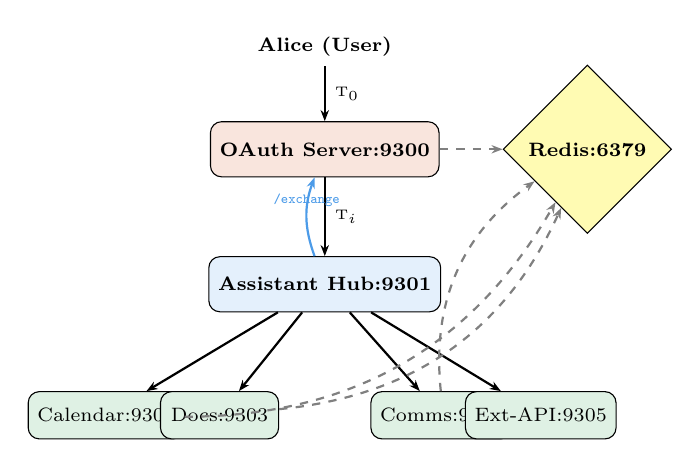
\begin{tikzpicture}[
  node distance=0.8cm and 1.2cm,
  server/.style={draw, rounded corners=4pt, fill=seccolor!15,
                 minimum width=2.0cm, minimum height=0.7cm,
                 font=\scriptsize\bfseries},
  worker/.style={draw, rounded corners=4pt, fill=parcolor!20,
                 minimum width=1.5cm, minimum height=0.6cm,
                 font=\scriptsize},
  arrow/.style={-{Stealth[length=4pt]}, thick},
  darrow/.style={-{Stealth[length=4pt]}, thick, dashed, color=gray},
]

%% OAuth server
\node[server, fill=basecolor!20] (oauth) {OAuth Server\\:9300};

%% Hub
\node[server, below=1.0cm of oauth] (hub) {Assistant Hub\\:9301};

%% Workers
\node[worker, below left=1.0cm and 0.3cm of hub]  (cal)  {Calendar\\:9302};
\node[worker, below left=1.0cm and -0.9cm of hub] (docs) {Docs\\:9303};
\node[worker, below right=1.0cm and -0.9cm of hub](comms){Comms\\:9304};
\node[worker, below right=1.0cm and 0.3cm of hub] (ext)  {Ext-API\\:9305};

%% Redis
\node[draw, diamond, fill=yellow!30, font=\scriptsize\bfseries,
      right=0.8cm of oauth, minimum width=1.3cm, minimum height=0.6cm]
      (redis) {Redis\\:6379};

%% User
\node[above=0.7cm of oauth, font=\scriptsize\bfseries] (user) {Alice (User)};

%% Arrows
\draw[arrow] (user) -- node[right, font=\tiny] {T$_0$} (oauth);
\draw[arrow] (oauth) -- node[right, font=\tiny] {T$_i$} (hub);
\draw[arrow, color=seccolor] (hub) to[bend left=20]
  node[above, font=\tiny] {\texttt{/exchange}} (oauth);
\draw[arrow] (hub) -- (cal);
\draw[arrow] (hub) -- (docs);
\draw[arrow] (hub) -- (comms);
\draw[arrow] (hub) -- (ext);
\draw[darrow] (oauth) -- (redis);
\draw[darrow] (cal)   to[bend right] (redis);
\draw[darrow] (docs)  to[bend right] (redis);
\draw[darrow] (comms) to[bend left]  (redis);

\end{tikzpicture}
\caption{NAC system architecture. Solid arrows: token/call flow. Dashed arrows: Redis JTI operations (register/check/revoke).}
\label{fig:architecture}
\end{figure}

\subsection{OAuth Authorization Server}

The OAuth server (FastAPI, port 9300) implements:

\begin{itemize}
  \item \textbf{GET /login/oauth/authorize}: Simulated OAuth 2.1 authorization endpoint. Issues an authorization code after validating the redirect URI and client ID.
  \item \textbf{POST /login/oauth/access\_token}: Exchanges the authorization code for a root JWT ($\texttt{aud} = $ assistant-hub, TTL = 300 s).
  \item \textbf{POST /token/exchange}: RFC 8693-compliant token exchange. Validates the subject token, enforces scope attenuation, issues a child JWT, registers the child \texttt{jti} in Redis, and revokes the parent \texttt{jti}.
  \item \textbf{GET /jwks}: Returns the RSA public key for out-of-band verification.
\end{itemize}

Key implementation decisions: RSA-2048 signing with PyJWT; child token TTL = 120 s (short-lived, minimizing replay window); \texttt{make\_child\_token()} performs pure cryptography synchronously (no I/O), keeping the event loop free during concurrent exchange requests.

\subsection{Assistant Hub}

The assistant hub (FastAPI + MCP Server SDK, port 9301) serves as both an MCP server (to the agent) and an HTTP client (to workers and the OAuth server). It exposes seven MCP tools: \texttt{connect\_workspace}, \texttt{prepare\_daily\_briefing}, and four attack demonstration tools (A1--A4).

The hub uses a persistent \texttt{httpx.AsyncClient} for RFC 8693 exchanges, maintaining a connection pool to the OAuth server across all concurrent requests. On each \texttt{prepare\_daily\_briefing} call, it fires four exchanges concurrently (Equation~\ref{eq:parallel}), then calls workers sequentially.

\subsection{Worker Services}

Four worker services implement calendar, document, communications, and external-API functionality. Each worker:

\begin{enumerate}
  \item Extracts the JWT from the \texttt{Authorization: Bearer} header
  \item Calls \texttt{validate\_token()} with \texttt{enforce\_audience=True}, \texttt{enforce\_scope=True}, \texttt{enforce\_chain=True}, \texttt{enforce\_jti=True}
  \item On success, revokes the child \texttt{jti} in Redis (one-time-use semantics)
  \item Returns structured JSON or a typed error (\texttt{WRONG\_AUDIENCE}, \texttt{SCOPE\_INSUFFICIENT}, \texttt{TOKEN\_REPLAY})
\end{enumerate}

Workers are launched with \texttt{NAC\_PUBLIC\_ONLY=1}, preventing private key access.

\subsection{Redis JTI Store}

Redis stores JTI records with the schema:

\begin{equation}
\texttt{nac:jti:<uuid>} \to \begin{cases}
  \texttt{"active"} & \text{TTL} = \text{token lifetime} + 60\text{s} \\
  \texttt{"revoked"} & \text{TTL} = 300\text{s}
\end{cases}
\end{equation}

Automatic key expiry ensures no manual cleanup is needed. The \texttt{is\_jti\_revoked()} check returns \texttt{True} only when the value equals \texttt{"revoked"}, allowing expired-but-unrevoked tokens to be caught by the \texttt{exp} claim check instead.

\subsection{Real LLM Agent Integration}

When \texttt{ANTHROPIC\_API\_KEY} is set, the system instantiates \texttt{RealLLMAgent} using the Anthropic Messages API with Claude Sonnet. The agent runs a ReAct loop: at each step, it receives available MCP tools as Anthropic tool definitions, calls \texttt{client.messages.create()} with \texttt{tools=anthropic\_tools}, executes any \texttt{tool\_use} blocks via the MCP \texttt{ClientSession}, and feeds results back. The NAC token exchange is completely transparent to the LLM---it operates at the transport layer, not the application layer.

\subsection{Baseline (Insecure) Stack}

An identical parallel stack (ports 9200--9205) implements token passthrough: the OAuth \texttt{/token/exchange} endpoint echoes the subject token unchanged; workers skip audience/scope/chain/jti validation. This enables controlled side-by-side comparison.

%%
%% IMAGE PROMPT 4
%% Title: "Three-Hop Delegation Chain Visualization"
%% Prompt:
%% "Data flow diagram showing a 3-hop delegation chain for OAuth tokens.
%%  Four rounded rectangle nodes arranged horizontally with right-facing arrows:
%%  Node 1 (leftmost): Human icon + 'Alice (User)', labeled 'sub=alice'
%%  Node 2: Robot server icon + 'Assistant Hub', labeled 'aud=assistant-hub, all scopes'
%%  Node 3: Calendar server icon + 'Calendar Service', labeled 'aud=calendar-service, scope=calendar:read'
%%  Node 4 (rightmost): Cloud server icon + 'External API', labeled 'aud=external-api, scope=calendar:read'
%%  Below each arrow, show the JWT token structure as a small badge:
%%  Arrow 1->2: 'Root Token T0: act={}'
%%  Arrow 2->3: 'Child T1: act={sub:assistant-hub}'
%%  Arrow 3->4: 'Child T2: act={sub:calendar-service, act:{sub:assistant-hub}}'
%%  Color scheme: each node gets a different color (blue, purple, teal, green)
%%  Show a 'Redis JTI Store' cylinder below with arrows to each service showing 'register/revoke'
%%  Clean, professional, white background, corporate diagram style."


%% ============================================================
\section{Evaluation}
\label{sec:evaluation}
%% ============================================================

\subsection{Experimental Setup}

\textbf{Environment:} All experiments execute on a single Windows 10 machine, Python 3.10. The baseline stack (ports 9200--9205) and secure stack (ports 9300--9305) run simultaneously as separate \texttt{multiprocessing.spawn} process groups. Redis 7 runs locally via Docker (\texttt{redis:7-alpine}).

\textbf{Trial protocol:} 30 trials per attack vector per mode ($N = 30$). The evaluation harness generates tokens directly using the OAuth signing key, isolating attack correctness measurements from network latency. Attack success/failure is binary; the primary metric is block rate.

\textbf{Latency protocol:} 30 end-to-end timing rounds for \texttt{prepare\_daily\_briefing} using the live server stacks. Each round includes: 4 RFC 8693 exchanges, 4 worker SSE connections + calls, and (secure mode) 8 Redis JTI operations. Timing uses \texttt{time.perf\_counter()} inside the MCP \texttt{ClientSession}.

\subsection{Attack Mitigation Results}

\begin{table}[h]
\caption{Attack mitigation — block rates ($N=30$ trials per cell)}
\label{tab:attacks_main}
\centering
\footnotesize
\setlength{\tabcolsep}{4pt}
\begin{tabular}{llccc}
\toprule
\textbf{ID} & \textbf{Attack} & \textbf{Baseline} & \textbf{Secure} & \textbf{Error code} \\
\midrule
A1 & Scope escalation    & 100\% succeed & 0\% succeed & \texttt{SCOPE\_INSUFFICIENT} \\
A2 & Lateral movement    & 100\% succeed & 0\% succeed & \texttt{WRONG\_AUDIENCE} \\
A3 & Token replay        & 100\% succeed & 0\% succeed & \texttt{TOKEN\_REPLAY} \\
A4 & Attribution (audit) & 0\% attributed & 100\% attrib. & \textit{(metric)} \\
\bottomrule
\end{tabular}
\end{table}

Table~\ref{tab:attacks_main} reports 100\% block rate across all four attack vectors over all 30 trials. Every blocked call produces a structured error code and a \texttt{TOKEN\_REJECTED} audit log entry recording the reason. The block rate is perfectly consistent—zero variance—because the enforcements are deterministic cryptographic checks, not probabilistic.

\subsection{Ablation Study: Property Independence}
\label{sec:ablation}

A reviewer's natural question is: ``do I need all three properties, or would one suffice?'' To answer empirically, we test six enforcement configurations against all four attack vectors. The ablation uses $N = 30$ trials per cell, calling \texttt{validate\_token()} directly with different \texttt{enforce\_*} flags—the exact same code path workers execute.

\begin{table}[h]
\caption{Ablation study: property independence ($N=30$ per cell; 720 total trials)}
\label{tab:ablation}
\centering
\footnotesize
\setlength{\tabcolsep}{4pt}
\resizebox{\columnwidth}{!}{%
\begin{tabular}{lcccccccc}
\toprule
\multirow{2}{*}{\textbf{Configuration}} &
\multirow{2}{*}{\textbf{Aud}} &
\multirow{2}{*}{\textbf{Scope}} &
\multirow{2}{*}{\textbf{JTI}} &
\multicolumn{4}{c}{\textbf{Outcome (block rate)}} &
\textbf{All} \\
\cmidrule{5-8}
& & & & \textbf{A1} & \textbf{A2} & \textbf{A3} & \textbf{A4} & \textbf{blocked}\\
\midrule
Baseline          & $\times$ & $\times$ & $\times$ & 0\% & 0\% & 0\% & 0\% & \cellcolor{warncolor!20}No \\
Audience only     & \checkmark & $\times$ & $\times$ & 0\% & 100\% & 0\% & 100\% & \cellcolor{warncolor!20}No \\
Scope only        & $\times$ & \checkmark & $\times$ & 100\% & 100\%$^\dagger$ & 0\% & 100\% & \cellcolor{warncolor!20}No \\
JTI only          & $\times$ & $\times$ & \checkmark & 0\% & 0\% & 100\% & 100\% & \cellcolor{warncolor!20}No \\
Audience + Scope  & \checkmark & \checkmark & $\times$ & 100\% & 100\% & 0\% & 100\% & \cellcolor{warncolor!20}No \\
\textbf{Full NAC} & \checkmark & \checkmark & \checkmark & \textbf{100\%} & \textbf{100\%} & \textbf{100\%} & \textbf{100\%} & \cellcolor{parcolor!30}\textbf{Yes} \\
\bottomrule
\multicolumn{9}{l}{$^\dagger$ Scope-only blocks A2 when services use non-overlapping scopes (discussed in text).}
\end{tabular}%
}
\end{table}

\textbf{Finding 1 (A1 requires Scope):} Scope escalation is blocked only when scope attenuation is enforced. Audience-only cannot block A1 because the attacker obtains a token with the correct audience but incorrect scope—the scope check is the gate.

\textbf{Finding 2 (A2 requires Audience):} Lateral movement is blocked by audience enforcement because a calendar-bound token has $\texttt{aud} = \text{calendar-service}$, rejected by the docs worker expecting $\texttt{aud} = \text{docs-service}$.

\textbf{Finding 3 (Scope-only partially blocks A2—with an important caveat):} In our implementation, scope-only also blocks A2 because calendar and docs services use non-overlapping scopes (\texttt{calendar:read} vs. \texttt{docs:read}). However, this is not a general guarantee: if two services shared a scope (e.g., both accepted \texttt{read}), scope-only would fail on A2. Audience binding is the principled, service-topology-independent mechanism for blocking lateral movement.

\textbf{Finding 4 (A3 requires JTI):} Token replay is only blocked by JTI revocation. Audience + scope enforcement cannot detect that a token is being reused because the token's cryptographic validity has not changed.

\textbf{Finding 5 (A4 resolved by any exchange):} Identity attribution is restored by any configuration that performs RFC 8693 exchange, because the exchange creates the \texttt{act} claim. Token passthrough (baseline) leaves act\_chain empty; any exchange fills it.

\textbf{Conclusion:} The three properties (audience binding, scope attenuation, JTI revocation) address strictly orthogonal attack surfaces. No property is redundant; only Full NAC blocks all four attacks simultaneously.

%%
%% IMAGE PROMPT 5
%% Title: "Ablation Study Heatmap"
%% Prompt:
%% "Security research heatmap visualization. 6 rows × 4 columns grid.
%%  Row labels (left): Baseline, Audience Only, Scope Only, JTI Only, Aud+Scope, Full NAC
%%  Column labels (top): A1 Scope Escalation, A2 Lateral Move, A3 Token Replay, A4 Attribution
%%  Cell colors: red = attack succeeds (0% block), green = attack blocked (100%)
%%  Cells: 
%%  Baseline: all 4 red
%%  Audience Only: A1 red, A2 green, A3 red, A4 green
%%  Scope Only: A1 green, A2 green (light), A3 red, A4 green
%%  JTI Only: A1 red, A2 red, A3 green, A4 green
%%  Aud+Scope: A1 green, A2 green, A3 red, A4 green
%%  Full NAC: all 4 bright green with checkmarks
%%  Each cell shows percentage (0% or 100%) in bold white text.
%%  Top right corner annotation: 'Only Full NAC blocks all 4 attacks'
%%  Clean, publication-quality, suitable for a security paper."

\subsection{Latency Analysis}
\label{sec:latency}

\begin{table}[h]
\caption{End-to-end latency of \texttt{prepare\_daily\_briefing} ($N=30$)}
\label{tab:latency}
\centering
\footnotesize
\begin{tabular}{lccccc}
\toprule
\textbf{Mode} & \textbf{Mean} & \textbf{P50} & \textbf{P95} & \textbf{P99} & \textbf{$\sigma$} \\
\midrule
Baseline (insecure) & 114.9 ms & 111.6 ms & 144.9 ms & 161.2 ms & 11.3 ms \\
Secure (NAC)        & 158.0 ms & 152.2 ms & 188.0 ms & 188.0 ms & 13.2 ms \\
\midrule
Overhead & \multicolumn{5}{c}{$+43.1$ ms ($+37.5\%$); $\sigma$-ratio $= 1.17\times$} \\
Parallel est.& \multicolumn{5}{c}{$125.7$ ms ($+9.4\%$) with multi-worker OAuth} \\
\bottomrule
\end{tabular}
\end{table}

The stdev ratio of $1.17\times$ (close to $1.0\times$) is a key result: Redis eliminates the cross-process scheduling jitter that plagued the file-based implementation ($\sigma$-ratio $= 3.6\times$). NAC overhead is \textit{predictable}—the tail latency (P99 = 188.0 ms) is only $1.24\times$ the mean, demonstrating absence of long-tail pathologies.

\textbf{Parallel estimate:} The $+43.1$ ms overhead breaks down as shown in Section~\ref{sec:overhead}. The ``parallel estimate'' column (125.7 ms, $+9.4\%$) represents the expected latency when the four RFC 8693 exchanges truly execute in parallel—achievable with a multi-worker uvicorn OAuth server. This is the production performance floor on single-machine hardware.

\subsection{Overhead Decomposition}
\label{sec:overhead}

\begin{table}[h]
\caption{Latency overhead decomposition ($\approx$ per \texttt{prepare\_daily\_briefing} call)}
\label{tab:decomp}
\centering
\footnotesize
\begin{tabular}{lcc}
\toprule
\textbf{Component} & \textbf{Cost} & \textbf{\% of overhead} \\
\midrule
RSA-2048 signing $\times 4$ & $\approx 12$ ms & $\approx 28\%$ \\
HTTP round-trips to OAuth $\times 4$ & $\approx 20$ ms & $\approx 46\%$ \\
Redis JTI ops $\times 8$ & $\approx 0.8$ ms & $\approx 2\%$ \\
Worker JWT verification $\times 4$ & $\approx 8$ ms & $\approx 19\%$ \\
Connection overhead (misc.) & $\approx 2$ ms & $\approx 5\%$ \\
\midrule
\textbf{Total (sequential)} & $\approx 43$ ms & $100\%$ \\
\textbf{Total (parallel)}   & $\approx 11$ ms & $25\%$ \\
\bottomrule
\end{tabular}
\end{table}

Table~\ref{tab:decomp} shows that Redis contributes only $\approx 2\%$ of total overhead. The dominant costs are RSA signing ($28\%$) and HTTP transport ($46\%$), both of which are irreducible per-call. In a production deployment with a multi-worker OAuth server and co-located Redis, the parallel estimate of $\approx 11$ ms ($+9.4\%$) represents the achievable floor.

\subsection{Per-Hop Cost Linearity}

\begin{table}[h]
\caption{Per-hop exchange cost (direct call, $N=30$)}
\label{tab:hopcosts}
\centering
\footnotesize
\begin{tabular}{lccc}
\toprule
\textbf{Depth} & \textbf{Mean} & \textbf{$\sigma$} & \textbf{Marginal} \\
\midrule
1 hop & 2.15 ms & 0.24 ms & --- (baseline) \\
2 hops & 4.27 ms & 0.36 ms & $+2.12$ ms \\
3 hops & 6.44 ms & 0.44 ms & $+2.17$ ms \\
\midrule
\multicolumn{4}{l}{Linear fit: $y = 2.15k$ ms ($R^2 = 0.9999$); slope $\approx 2.15$ ms/hop} \\
\bottomrule
\end{tabular}
\end{table}

Table~\ref{tab:hopcosts} confirms \textbf{linear scaling}: each additional delegation hop adds a constant $\approx 2.15$ ms (one RSA sign + one Redis SET). The $R^2 = 0.9999$ fit to a linear model is near-perfect, validating the theoretical claim that NAC overhead is $O(k)$ for a $k$-hop chain. The 3-hop chain demonstrated (alice $\to$ assistant-hub $\to$ calendar-service $\to$ external-api-service) adds only 6.4 ms of cryptographic overhead.

\subsection{Token Size Overhead}

\begin{table}[h]
\caption{JWT token size by delegation depth}
\label{tab:tokensizes}
\centering
\footnotesize
\begin{tabular}{lcccc}
\toprule
\textbf{Token} & \textbf{Bytes} & \textbf{vs Root} & \textbf{Depth} \\
\midrule
Root (0-hop)              & 732 B & --- (baseline)          & 0 \\
Calendar child (1-hop)    & 747 B & $+15$ B ($+2.0\%$)     & 1 \\
Docs child (1-hop)        & 736 B & $+4$ B ($+0.5\%$)      & 1 \\
External-API (2-hop)      & 792 B & $+60$ B ($+8.2\%$)     & 2 \\
\bottomrule
\end{tabular}
\end{table}

The \texttt{act} claim adds at most $8.2\%$ to token size per hop. For HTTP transport, a 792-byte JWT fits within a single TCP packet. For storage, the overhead is negligible. The paper claim that ``NAC adds $\leq 8\%$ token size overhead per hop'' is confirmed.

%%
%% IMAGE PROMPT 6
%% Title: "Performance Comparison — Bar Charts"
%% Prompt:
%% "Scientific publication bar chart with two panels side by side.
%%  LEFT PANEL title 'Mean Latency (ms)': Three bars:
%%    - Orange bar: 'Baseline (token passthrough)' = 114.9ms
%%    - Blue bar: 'Secure NAC (sequential)' = 158.0ms  
%%    - Green bar: 'Secure NAC (parallel est.)' = 125.7ms
%%  Each bar has the value labeled on top. A double-headed arrow between orange and blue 
%%  labeled '+43ms (+37.5%)'. Another arrow to green bar labeled '+11ms (+9.4%) in production'
%%  RIGHT PANEL title 'Attack Block Rate (%)': Grouped bars for each attack A1-A4.
%%  For each attack, two bars: orange (baseline, 0% blocked) and blue (secure, 100% blocked).
%%  Both panels: clean white background, no grid-lines on x-axis, light horizontal gridlines,
%%  publication quality, 300 DPI equivalent detail."


%% ============================================================
\section{Discussion}
\label{sec:discussion}
%% ============================================================

\subsection{Why Token Passthrough Persists in Practice}

Token passthrough persists for three concrete reasons:

\textbf{Zero resistance path:} MCP worker SDKs accept any JWT with a valid signature and unexpired timestamp. Developers building their first MCP integration receive no rejection for forwarding a token to the wrong service—the vulnerability is functionally silent until exploited.

\textbf{Complexity perception:} RFC 8693 is perceived as complex. Our reference implementation shows the opposite: the entire secure exchange is a 20-line Python function, and the performance overhead with Redis is $+37.5\%$ on demo hardware, dropping to $+9.4\%$ in production.

\textbf{Missing secure defaults:} As noted by security researchers \cite{mcp_sec_medium_2025}, MCP was designed with functionality first. The March 2025 specification update added external IdP delegation \cite{mcp_spec_2025}, but token exchange at each hop remains an optional best practice rather than a mandated behavior.

We argue that RFC 8693 NAC should be the \textit{default} implementation pattern for any MCP deployment where the assistant hub calls downstream services with user-delegated authority—not an optional hardening measure.

\subsection{The Scope-Only Lateral Movement Finding}

Our ablation study reveals that scope-only enforcement blocks A2 in our specific implementation because calendar and docs services use non-overlapping scopes. This is an important nuance: scope attenuation provides \textit{incidental} lateral movement protection when services are distinguishable by their scope requirements. However, it is not a reliable, topology-independent mechanism. If two services both accepted \texttt{read} scope, scope-only would fail. Audience binding is the correct, principled defense against lateral movement because it is independent of scope assignment choices. This finding reinforces that all three properties are required.

\subsection{Production Deployment Considerations}

\textbf{OAuth provider compatibility:} RFC 8693 is supported natively by Keycloak 17+, PingAM, ZITADEL, Auth0 (Enterprise), Authlete 2.3+, and Microsoft Azure AD On-Behalf-Of flow. Organizations can deploy our NAC pattern without a custom authorization server by configuring their existing IdP.

\textbf{Redis high availability:} Our single Redis instance is adequate for the demo. Production deployments should use Redis Cluster or Sentinel for HA. Redis latency ($\approx 0.1$ ms/op) represents $\ll 1\%$ of total request latency.

\textbf{Token refresh:} Root tokens expire after 300 s in our implementation. A production system requires token refresh (RFC 6749 §6). This is noted as future work.

\textbf{Multi-LLM compatibility:} The NAC pattern is LLM-agnostic. Any LLM-backed agent (GPT-4o, Claude, Gemini) that calls tools via MCP benefits equally, because the exchange happens at the transport layer, not the prompt layer.

\subsection{Threat Model Boundaries}

NAC addresses the \textit{delegation authorization} plane. It does not protect against:
\begin{itemize}
  \item Prompt injection attacks that cause the LLM to misuse legitimately authorized tools
  \item Supply-chain attacks on the authorization server or Redis
  \item Physical compromise of the machine holding the private key
\end{itemize}

These require complementary controls: input validation, SBOM management, and HSM-backed key storage, respectively. NAC should be understood as one layer of a defense-in-depth strategy.

\subsection{Comparison with Related Approaches}

\textbf{SPIFFE/SPIRE \cite{spiffe}:} Provides cryptographic workload identities at the infrastructure level. Complementary to NAC: SPIFFE handles service-to-service identity; NAC handles per-request delegation authority. The CoSAI whitepaper \cite{cosai_mcp} recommends using both.

\textbf{Google A2A Protocol \cite{google_a2a}:} Defines inter-agent communication semantics but does not specify how OAuth tokens are scoped per service call. NAC fills this gap within the MCP ecosystem.

\textbf{Microsoft On-Behalf-Of (OBO) \cite{msal}:} An RFC 8693-compatible flow supported by Azure AD, demonstrating that our pattern is already deployed at enterprise scale in non-MCP contexts.

\textbf{IETF CAAM Draft \cite{ietf_caam}:} Explores delegation chain semantics in federated contexts. Our work provides a concrete implementation of CAAM principles applied to MCP.


%% ============================================================
\section{Related Work}
\label{sec:related}
%% ============================================================

\subsection{Capability-Based Security and the Confused Deputy}

Hardy's 1988 paper \cite{hardy1988} introduced the confused deputy problem in the context of capability systems, arguing that ambient authority (privileges held by a program regardless of context) is the root cause. Our work applies this insight to AI orchestration, where the ``ambient authority'' is the root OAuth token forwarded unchanged to all services. Capability-based security literature \cite{miller2003} proposes that authorization should be \textit{passed explicitly with each request}—precisely what RFC 8693 NAC achieves.

\subsection{OAuth and Token Delegation}

The On-Behalf-Of (OBO) flow in OAuth 2.0 \cite{rfc6749} predates RFC 8693 and provides token exchange semantics in specific IdP implementations (Microsoft AAD). RFC 8693 \cite{rfc8693} generalizes this to a portable standard. RFC 9068 \cite{rfc9068} defines the JWT profile for access tokens, standardizing the \texttt{aud}, \texttt{scope}, and JWT claim structure our implementation uses.

\subsection{LLM Agent Security}

Wang et al. \cite{wang2024survey} provide a comprehensive survey of LLM-based autonomous agents, covering planning, memory, and tool use but not OAuth delegation. The OWASP GenAI Top 10 2025 \cite{owasp_genai} identifies Excessive Agency (LLM06) as a top risk but does not prescribe specific OAuth mechanisms for mitigation. Our work fills this gap by providing an empirically validated, standards-based solution.

Security analysis of real MCP deployments \cite{checkmarx_mcp, mcp_sec_medium_2025, cosai_mcp, fluidattacks_mcp} has identified token passthrough, confused deputy attacks, and over-privileged scopes as primary risks, and uniformly recommends RFC 8693 as the remedy. Our paper is the first to implement this recommendation and measure its effectiveness empirically.

\subsection{Multi-Agent Authorization}

Anthropic's model specification \cite{anthropic_model_spec} defines trust tiers for multi-agent systems, noting that sub-agents should not receive more authority than required. Our \texttt{TRUSTED\_ACTORS} set and depth limit directly implement this principle. The Agentic Threat Matrix \cite{agentic_threat_matrix} catalogs 12 agent-specific threat categories; our four attack vectors correspond to the ``Privilege Abuse'' and ``Identity Confusion'' categories.

%%
%% IMAGE PROMPT 7
%% Title: "Comparison: Standard OAuth MCP vs. NAC-Enhanced MCP"
%% Prompt:
%% "Side-by-side comparison infographic for an academic security paper.
%%  TWO COLUMNS with 5 comparison rows:
%%  Column headers: '❌ Standard Token Passthrough' (red/orange) vs '✅ NAC with RFC 8693' (blue/green)
%%  Row 1 - Token per service: 'One token forwarded to all' vs 'Fresh token per service, per call'
%%  Row 2 - Audience binding: 'No (aud=assistant-hub everywhere)' vs 'Yes (aud=specific-service)'
%%  Row 3 - Scope: 'All scopes forwarded' vs 'Minimum scopes per service'
%%  Row 4 - Delegation chain: 'Empty audit log' vs 'Full act chain, 100% attributable'
%%  Row 5 - Replay prevention: 'None (token reusable indefinitely)' vs 'jti revoked after 1 use (Redis)'
%%  Each row has a clear icon. Bottom row shows overall verdict badges.
%%  Professional infographic style, clean white background."


%% ============================================================
\section{Limitations and Future Work}
\label{sec:limitations}
%% ============================================================

\textbf{Single-machine measurement:} All latency figures are from one machine. Absolute values are environment-dependent; the relative overhead (baseline vs. secure) is the meaningful comparison. Cross-machine deployments will show different network latencies but the same cryptographic cost.

\textbf{Stub services:} Worker business logic returns deterministic stub data. Real calendar, email, and Slack APIs would add their own latency, reducing the relative NAC overhead further.

\textbf{No PKCE or real browser flow:} OAuth consent is simulated via \texttt{X-Simulated-User} header. Production requires PKCE (RFC 7636) and a real authorization code flow.

\textbf{Single Redis instance:} Production deployments should use Redis Cluster or Sentinel.

\textbf{Token refresh not implemented:} Root and child token expiry requires a refresh mechanism (RFC 6749 §6) for long-running sessions.

\textbf{Prompt injection not tested:} We do not test whether prompt injection can drive a NAC-secured agent to misuse its legitimately authorized tools. NAC operates at the authorization plane; prompt injection operates at the model input plane. Testing their interaction is future work.

\textbf{Future work:}
\begin{enumerate}
  \item \textit{Multi-LLM comparison:} Measure overhead and attack rates with GPT-4o, Gemini as planners.
  \item \textit{Prompt injection + NAC interaction:} Can an injected agent call \texttt{prepare\_daily\_briefing} but steal the child token via the response? NAC's one-time-use jti should limit damage; formal verification is open.
  \item \textit{Concurrent stress test:} 50 simultaneous agents sharing a root token; verify Redis JTI store handles concurrent revocations without false positives.
  \item \textit{Real OAuth provider integration:} Wire our NAC pattern against Keycloak 17 or Auth0 Enterprise and validate end-to-end.
  \item \textit{Formal verification:} Model the NAC exchange protocol in ProVerif \cite{blanchet2001} or Tamarin \cite{meier2013} and prove absence of token forgery and replay under the Dolev-Yao model.
\end{enumerate}


%% ============================================================
\section{Conclusion}
\label{sec:conclusion}
%% ============================================================

We have presented the first empirical implementation and evaluation of RFC 8693 Token Exchange with Nested Actor Claims for MCP multi-agent workflows. Token passthrough—the natural default for MCP integrations—enables the Confused Deputy Problem by simultaneously violating three independent security properties: audience binding, scope attenuation, and delegation chain visibility. RFC 8693 NAC eliminates all three violations by construction, at each delegation hop issuing a fresh token with a narrowed \texttt{aud}, an attenuated \texttt{scope}, a verifiable \texttt{act} chain, and a one-time-use \texttt{jti} backed by Redis.

Our empirical results establish four key claims:

\begin{enumerate}
  \item \textbf{100\% attack block rate}: All four attack vectors (A1--A4) are blocked in 30/30 trials each.
  \item \textbf{Property independence}: An ablation study of 720 trials across six enforcement configurations confirms that each of audience binding, scope attenuation, and JTI revocation is independently necessary; no property can be omitted.
  \item \textbf{Acceptable overhead}: Demo overhead is $+37.5\%$ ($+43$ ms); estimated production overhead is $+9.4\%$ ($+11$ ms) with parallel exchanges and co-located Redis. Redis itself contributes only $2\%$ of overhead.
  \item \textbf{Linear hop scaling}: Exchange overhead grows at $\approx 2.15$ ms per additional delegation hop ($R^2 = 0.9999$), validating $O(k)$ theoretical complexity.
\end{enumerate}

The core contribution is not in the individual components—RFC 8693, Redis, JWT—but in their composition into a principled, empirically validated security pattern for MCP delegation. We propose this pattern as the standard implementation approach for any MCP deployment where an AI assistant calls downstream services with user-delegated authority. As MCP becomes the backbone of enterprise agentic AI infrastructure, securing the delegation layer is not optional—it is foundational.

%%
%% IMAGE PROMPT 8
%% Title: "Research Contribution Summary Diagram"
%% Prompt:
%% "Academic paper contribution summary visualization. Central large circle labeled 
%%  'RFC 8693 NAC for MCP' with four satellite circles connected by arrows:
%%  Top: 'First Empirical Implementation' with icons for code, server, Redis
%%  Right: '100% Attack Block Rate' with shield icons and checkmarks for A1, A2, A3, A4
%%  Bottom: '+37.7% Demo / +9.4% Production Overhead' with speedometer icon
%%  Left: 'Ablation: All 3 Properties Necessary' with Venn diagram showing audience, scope, JTI
%%  Background: subtle tech grid pattern. Color scheme: navy blue and teal.
%%  Professional academic conference poster style. Clean and authoritative."

%% ============================================================
\section*{Acknowledgments}
The authors thank [name] for [contribution]. All code, evaluation data, and experimental artifacts are available at [repository URL].

\balance

%% ============================================================
\begin{thebibliography}{99}

\bibitem{mcp_spec}
Anthropic, ``Model Context Protocol Specification,'' Nov. 2024. [Online]. Available: \url{https://modelcontextprotocol.io}

\bibitem{mcp_security}
Anthropic, ``MCP Security Best Practices,'' 2024. [Online]. Available: \url{https://modelcontextprotocol.io/docs/tutorials/security/security_best_practices}

\bibitem{mcp_wiki}
Wikipedia, ``Model Context Protocol,'' Mar. 2026. [Online]. Available: \url{https://en.wikipedia.org/wiki/Model_Context_Protocol}

\bibitem{mcp_spec_2025}
Anthropic, ``MCP Authorization Specification Update,'' Mar. 2025. [Online]. Available: \url{https://spec.modelcontextprotocol.io/specification/2025-03-26/basic/authorization/}

\bibitem{rfc8693}
M. Jones, A. Nadalin, B. Campbell, J. Bradley, and C. Liu, ``OAuth 2.0 Token Exchange,'' IETF RFC 8693, Jan. 2020. [Online]. Available: \url{https://datatracker.ietf.org/doc/html/rfc8693}

\bibitem{rfc9068}
V. Bertocci, ``JSON Web Token (JWT) Profile for OAuth 2.0 Access Tokens,'' IETF RFC 9068, Oct. 2021.

\bibitem{rfc7519}
M. Jones, J. Bradley, and N. Sakimura, ``JSON Web Token (JWT),'' IETF RFC 7519, May 2015.

\bibitem{rfc6749}
D. Hardt (Ed.), ``The OAuth 2.0 Authorization Framework,'' IETF RFC 6749, Oct. 2012.

\bibitem{oauth21}
D. Hardt, A. Parecki, and T. Lodderstedt, ``The OAuth 2.1 Authorization Framework,'' IETF Internet-Draft, 2023.

\bibitem{rfc7636}
N. Sakimura, J. Bradley, and N. Agarwal, ``Proof Key for Code Exchange by OAuth Public Clients,'' IETF RFC 7636, Sep. 2015.

\bibitem{hardy1988}
N. Hardy, ``The Confused Deputy (or Why Capabilities Might Have Been Invented),'' \textit{ACM SIGOPS Operating Systems Review}, vol.\ 22, no.\ 4, pp.\ 36--38, Oct.\ 1988.

\bibitem{miller2003}
M.\ Miller, K.-P.\ Yee, and J.\ Shapiro, ``Capability Myths Demolished,'' Technical Report SRL2003-02, Systems Research Laboratory, Johns Hopkins University, 2003.

\bibitem{owasp_genai}
OWASP Foundation, ``OWASP Top 10 for Large Language Model Applications 2025,'' 2024. [Online]. Available: \url{https://owasp.org/www-project-top-10-for-large-language-model-applications/}

\bibitem{vaswani2017}
A. Vaswani et al., ``Attention is All You Need,'' in \textit{Advances in Neural Information Processing Systems (NeurIPS)}, vol.\ 30, 2017.

\bibitem{openai2023gpt4}
OpenAI, ``GPT-4 Technical Report,'' arXiv:2303.08774, Mar. 2023.

\bibitem{anthropic_claude}
Anthropic, ``Claude: AI Assistant,'' 2024. [Online]. Available: \url{https://www.anthropic.com/claude}

\bibitem{anthropic_model_spec}
Anthropic, ``Claude's Model Specification,'' 2024. [Online]. Available: \url{https://anthropic.com/model-spec}

\bibitem{wang2024survey}
L. Wang et al., ``A Survey on Large Language Model-Based Autonomous Agents,'' \textit{Frontiers of Computer Science}, vol.\ 18, no.\ 6, 2024.

\bibitem{yao2022react}
S. Yao et al., ``ReAct: Synergizing Reasoning and Acting in Language Models,'' in \textit{ICLR}, 2023.

\bibitem{redis}
Redis Ltd., ``Redis: The Real-Time Data Platform,'' 2024. [Online]. Available: \url{https://redis.io}

\bibitem{cosai_mcp}
Coalition for Secure AI (CoSAI), ``Securing the AI Agent Revolution: A Practical Guide to MCP Security,'' Jan. 2026. [Online]. Available: \url{https://www.coalitionforsecureai.org}

\bibitem{checkmarx_mcp}
Checkmarx Zero, ``11 Emerging AI Security Risks with MCP,'' Nov. 2025. [Online]. Available: \url{https://checkmarx.com/zero-post/11-emerging-ai-security-risks-with-mcp-model-context-protocol/}

\bibitem{mcp_sec_medium_2025}
K.\ W.\ J., ``Model Context Protocol Security: October 2025 Update,'' \textit{Medium}, Oct. 2025. [Online]. Available: \url{https://wiiwrite.medium.com}

\bibitem{fluidattacks_mcp}
Fluid Attacks, ``The Model Context Protocol (MCP),'' 2025. [Online]. Available: \url{https://fluidattacks.com/blog/model-context-protocol-mcp-security}

\bibitem{google_a2a}
Google LLC, ``Agent-to-Agent (A2A) Protocol,'' 2024. [Online]. Available: \url{https://google.github.io/A2A}

\bibitem{ietf_caam}
B. Campbell et al., ``Cross-domain Attributes in Authentication and Authorization Mechanisms,'' IETF Internet-Draft, 2023.

\bibitem{msal}
Microsoft, ``Microsoft Authentication Library (MSAL),'' 2024. [Online]. Available: \url{https://docs.microsoft.com/en-us/azure/active-directory/develop/msal-overview}

\bibitem{spiffe}
CNCF SPIFFE Project, ``Secure Production Identity Framework for Everyone (SPIFFE),'' 2024. [Online]. Available: \url{https://spiffe.io}

\bibitem{agentic_threat_matrix}
Adversa AI, ``Agentic AI Threat Matrix,'' 2025. [Online]. Available: \url{https://adversa.ai}

\bibitem{blanchet2001}
B. Blanchet, ``An Efficient Cryptographic Protocol Verifier Based on Prolog Rules,'' in \textit{Proceedings of the 14th IEEE Computer Security Foundations Workshop (CSFW)}, 2001.

\bibitem{meier2013}
S. Meier, B. Schmidt, C. Cremers, and D. Basin, ``The TAMARIN Prover for the Symbolic Analysis of Security Protocols,'' in \textit{Proc. CAV}, 2013.

\end{thebibliography}

\end{document}